\chapter{Zaključak}

Korištenjem \verb|NumPy| i \verb|Matplotlib| biblioteka u Pythonu, pomoću sljedećeg koda možemo dobiti 3D prikaz cijele multivarijatne funkcije:

\inputminted{python}{./code/graf_fje.py}

\begin{figure}
    \centering
    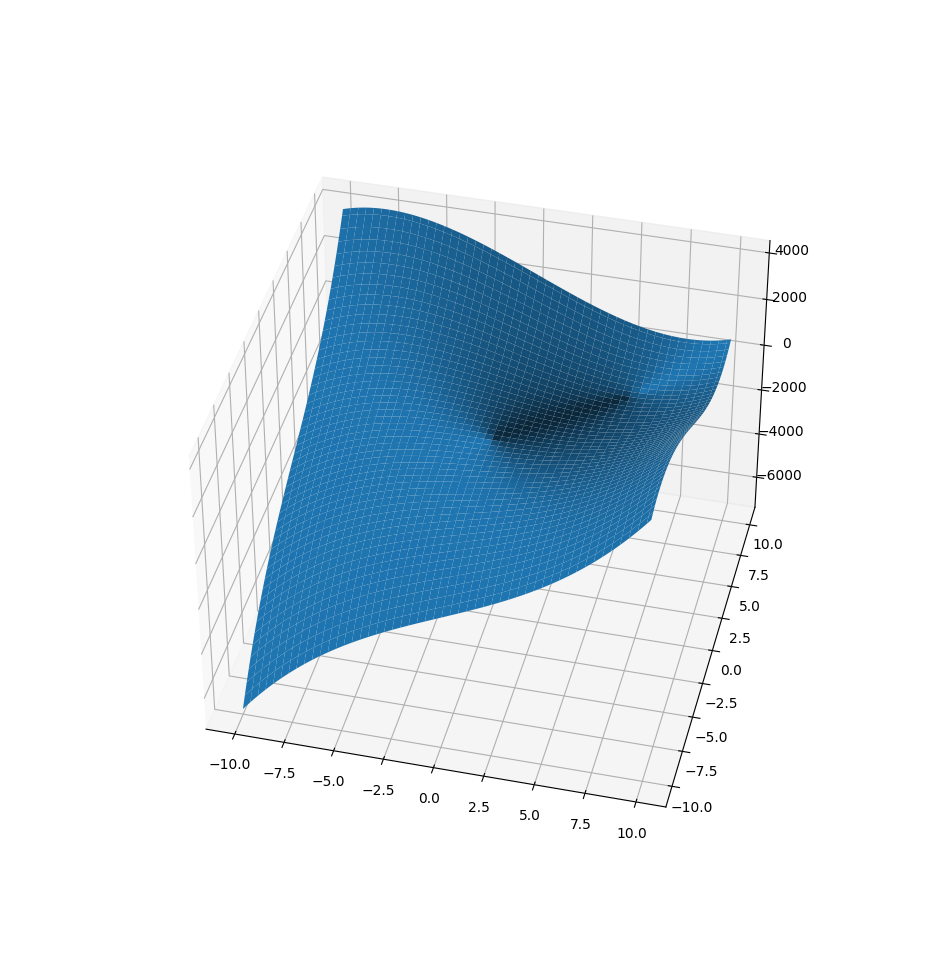
\includegraphics[width=0.8\textwidth]{graf_fje}
    \caption{Graf zadane funkcije $f$}
\end{figure}

Na grafu vidimo da dobivene točke jesu ekstremi funkcije. \par
Za algebarsko određivanje o kakvim se ekstremima radi bi trebali odrediti Hessovu matricu i parcijalne derivacije višeg reda \cite[][poglavlje 6.3]{ccalc}, no to nije traženo u sklopu ovog zadatka.

\newpage
